%!TEX root = ../main.tex

\section*{Confidential Compute - Known Vulnerabilities}
\addcontentsline{toc}{section}{Confidential Compute - Known Vulnerabilities}

This table is in addition to the table provided bij AMD previously mentioned.
This table only includes the literature mentioned in this chapter. 
The main conclusion is that the known vulnerabilities 
are to be mitigated in the SEV-SNP. 
The development team of AMD is really transparent on the found vulnerabilities 
and in many papers thanked for their collaboration 
on confirming the found vulnerabilities. 

\begin{table}[ht]
\label{lit}

\caption{Found literate on known vulnerabilities AMD EPYC confidential compute}
\centering
{
\footnotesize
  \begin{tabular}{|p{3.5cm}|p{3.5cm}|p{3.5cm}|p{3.5cm}|}
    \hline
     & \textbf{SEV} 
     & \textbf{SEV-ES} 
     & \textbf{SEV-SNP}\\
    \hline

    \textbf{to be sorted} 
    & \begin{minipage}[t]{7cm}
        \cite{hetzelt_security_2017}\\
        \cite{du_secure_2017} \\
        \cite{li_tlb_2021}
      \end{minipage}
    & \cite{li_tlb_2021} 
    & 
    \\

    \textbf{Physical attacks} 
    & \begin{minipage}[t]{7cm}
        \cite{li_exploiting_2019} \\
        \cite{buhren_insecure_2019} \\
        \cite{buhren_one_2021}
      \end{minipage}
    & \begin{minipage}[t]{7cm}
        \cite{wilke_sevurity_2020}\\
        \cite{buhren_one_2021} 
      \end{minipage}
    & \cite{buhren_one_2021}
    \\

    \textbf{Software attacks} 
    & \begin{minipage}[t]{7cm}
        \cite{morbitzer_severed_2018} \\
        \cite{2019-werner}\\
        \cite{hetzelt_via_2021}
      \end{minipage}
    & \begin{minipage}[t]{7cm}
        \cite{2019-werner}\\
        \cite{hetzelt_via_2021} 
       \end{minipage}
    & 
    \\

    \textbf{Side-channel attacks} 
    & \begin{minipage}[t]{7cm}
        \cite{li_crossline_2021}\\ 
        \cite{li_cipherleaks_2021}\\ 
        \cite{mestas_exploitation_2021} 
      \end{minipage}
    & \begin{minipage}[t]{7cm}
        \cite{li_crossline_2021}\\
        \cite{li_cipherleaks_2021}\\
        \cite{mestas_exploitation_2021} 
      \end{minipage}
    & 
    \\

    \textbf{Denial-of-service attacks} 
    & 
    & 
    & 
    \\
    \hline

  \end{tabular}
}
\end{table}

There are two authors that are very active in the discovery of the vulnerabilities. 
These two authors are: 
\begin{enumerate}
  \item \textbf{Mengyuan Li} from the Ohio State University.  
  \item \textbf{Robert Buhren} from T-Lab TU  Berlin.
\end{enumerate}

The abstract and the conclusion of each of the entries of tabel \ref{lit}
are included in the following sections.

The conclusion of the found literature can be found in the summary (\ref{summary}) of this document.

\newpage
\subsection{Academic Literature researches on AMD SEV}

\subsubsection{References found by \cite{2019-werner} }

TODO:  insert table insert data

\subsubsection{References found by \cite{leijonberg_viability_2021} }

\begin{itemize}
\item 14  \cite{buhren_insecure_2019}
\item 38  \cite{li_exploiting_2019}
\item 37  \cite{li_exploiting_2019}
\item 39  \cite{2019-werner}
\end{itemize}
See figure \ref{fig:classification-vulnerabilities}.

\begin{figure}[!ht]
    \centering
    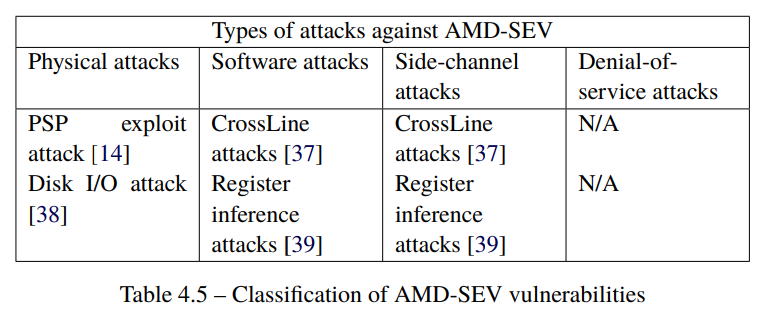
\includegraphics[width=0.6\linewidth]{classification-vulnerabilities}
    \caption{table with known AMD-SEV vulnerabilities  
    from \cite{leijonberg_viability_2021}}
    \label{fig:classification-vulnerabilities}
\end{figure}


\subsubsection{References found by \cite{li_crossline_2021} }
TODO:  insert data


\begin{figure}[!ht]
    \centering
    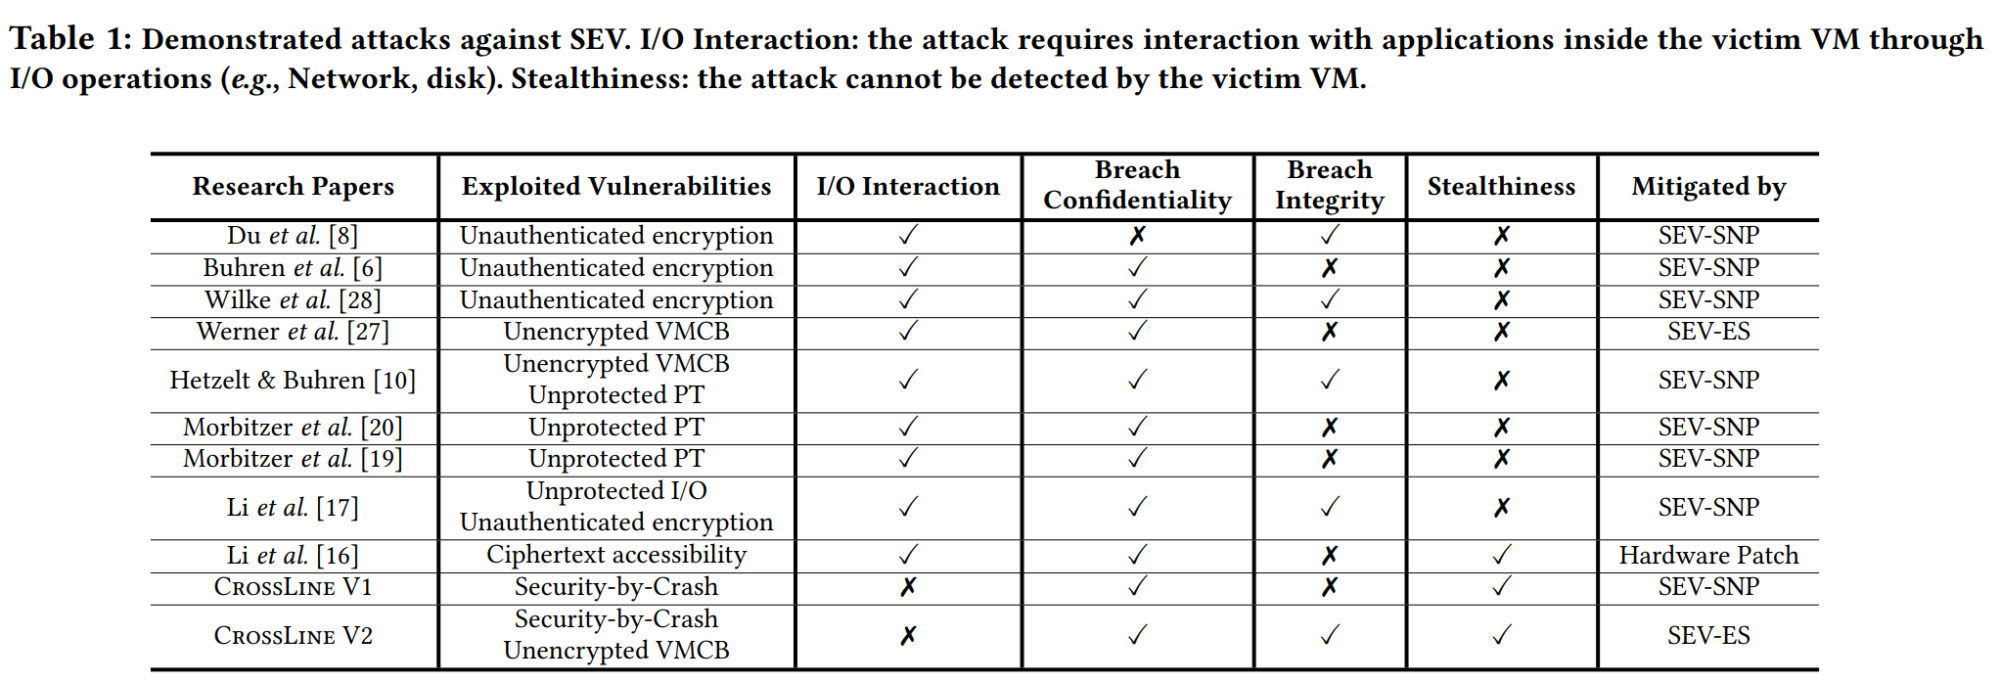
\includegraphics[width=1.1\linewidth]{classification-vulnerabilities-2}
    \caption{table with known AMD-SEV vulnerabilities  
    from \cite{li_crossline_2021}}
    \label{fig:classification-vulnerabilities-2}
\end{figure}

\newpage%!TEX root = ../main.tex

\subsection{\cite{du_secure_2017} - Secure Encrypted Virtualization is Unsecure}

\textbf{Secure Encrypted Virtualization is Unsecure}

\subsubsection*{Abstract \cite{du_secure_2017}}
“Virtualization has become more important since cloud computing is getting more and more popular than before. There’s an increasing demand for security among the cloud customers. AMD plans to provide Secure Encrypted Virtualization (SEV)[8] technology in its latest processor EPYC to protect virtual machines by encrypting its memory but without integrity protection. In this paper, we analyzed the weakness in the SEV design due to lack of integrity protection thus it is not so secure. Using different design flaw in physical address-based tweak algorithm to protect against ciphertext block move attacks, we found a realistic attack against SEV which could obtain the root privilege of an encrypted virtual machine protected by SEV. A demo to simulate the attack against a virtual machine protected by SEV is done in a Ryzen machine which supports Secure Memory Encryption (SME)[8] technology since SEV enabled machine is still not available in market.“

\subsubsection*{Conclusion \cite{du_secure_2017}}
“In this paper, we have demonstrated that the current implementation of SEV is vulnerable. We suggest AMD to update the physical address-based tweak algorithm before releasing SEV into market. The physical address-based tweak algorithm should not tweak the address into plaintexts or cipher-texts. The address should be tweaked into key of AES algorithm to protect against cipher-text move attacks. It is preferred that Key Derivation Function such as the one specified in NIST SP 800-108 [24] should be used to tweak the address into the key. Encryption is not enough to isolate VMs from hypervisor and it is better that integrity protection could also be provided. The idea to provide a technology to isolate data of guest VM from hypervisor is promising, but there’re still a lot of improvement opportunities in the current implementation.“

\newpage%!TEX root = ../main.tex

\subsection{\cite{hetzelt_security_2017} - Security Analysis of Encrypted Virtual Machines}

\textbf{Security Analysis of Encrypted Virtual Machines }

\subsubsection*{Abstract \cite{hetzelt_security_2017}}
“Both AMD and Intel have presented technologies 
for confidential computing in cloud environments. 
The proposed solutions — AMD SEV (-ES, -SNP) and Intel TDX — protect Virtual Machines (VMs) against attacks from higher privileged layers through memory encryption and integrity protection. 
This model of computation draws a new trust boundary between virtual devices and the VM, which insofar lacks thorough examination. 
In this paper, we therefore present an analysis of the virtual device interface and discuss several attack vectors against a protected VM. 
Further, we develop and evaluate VIA, an automated analysis tool to detect cases of improper sanitization of input received via the virtual device interface. 
VIA improves upon existing approaches for the automated analysis of device interfaces in the following aspects: 
(i) support for virtualization relevant buses, 
(ii) efficient Direct Memory Access (DMA) support and 
(iii) performance. 
VIA builds upon the Linux Kernel Library and clang’s libfuzzer to fuzz 
the communication between the driver and the device via MMIO, PIO, and DMA. 
An evaluation of VIA shows that it performs 570 executions per second on average 
and improves performance compared to existing approaches by an average factor of 2706.
 Using VIA, we analyzed 22 drivers in Linux 5.10.0-rc6, 
 thereby uncovering 50 bugs and initiating multiple patches to the virtual device driver interface of Linux. 
 To prove our findings’ criticality under the threat model of AMD SEV and Intel TDX, we showcase three exemplary attacks based on the bugs found. 
 The attacks enable a malicious hypervisor to corrupt the memory and gain code execution in protected VMs with SEV-ES and are theoretically applicable to SEV-SNP and TDX.”

\subsubsection*{Conclusion \cite{hetzelt_security_2017}}
“We presented VIA: a framework for dynamic analysis of drivers under the threat model of a malicious HV. VIA was applied to 22 drivers in Linux 5.10.0-rc6, which covered network drivers, VirtIObased drivers, and platform drivers. The evaluation found 50 bugs from a variety of classes and initiated multiple patches to the Linux kernel. We implement Proof-of-Concept exploits for three bug classes that gain code execution or corrupt memory inside an AMD SEV-ES VM. The described exploits demonstrate how the capabilities of a malicious HV, such as control over virtual devices, fine grained control over VM execution as well as information about the VM execution state, can be used to craft reliable exploits. The majority of bugs were reported to the driver maintainers, and the security implications were responsibly disclosed.

Unlike other solutions for driver analysis, VIA carefully considers the capabilities of the HV and the semantics of the DMA API to detect more cases of improper input sanitization and anti-patterns in device programming. VIA provides a coverage-driven in-process userspace fuzzer built upon libfuzzer and LKL. Compared to existing approaches, VIA reduces setup overhead by moving the analysis into a userspace program. In combination with targeted optimizations of the userspace kernel environment, VIA drastically improves dynamic analysis throughput. To the best of our knowledge, VIA presents the first approach to analyze the device driver interface under the new threat model of protected virtual machines.

Our results suggest that many Linux device drivers do not correctly sanitize device-provided data. Under the threat model of AMD SEV-SNP and Intel TDX, this presents a serious security risk for the protected VM, which may be exploited through a software driver bug. Thus, the software operating under such a threat model should reduce the interfaces with untrusted entities and should rely on established methods for testing the remaining interfaces.“


\newpage%!TEX root = ../main.tex

\subsection{\cite{morbitzer_severed_2018} - SEVered: Subverting AMD’s Virtual Machine Encryption}

\textbf{SEVered: Subverting AMD’s Virtual Machine Encryption}

\subsubsection*{Abstract \cite{morbitzer_severed_2018}}
“AMD SEV is a hardware feature designed for the secure encryption of virtual machines. SEV aims to protect virtual machine memory not only from other malicious guests and physical attackers, but also from a possibly malicious hypervisor. This relieves cloud and virtual server customers from fully trusting their server providers and the hypervisors they are using. We present the design and implementation of SEVered, an attack from a malicious hypervisor capable of extracting the full contents of main memory in plaintext from SEV-encrypted virtual machines. SEVered neither requires physical access nor colluding virtual machines, but only relies on a remote communication service, such as a web server, running in the targeted virtual machine. We verify the effectiveness of SEVered on a recent AMD SEV-enabled server platform running different services, such as web or SSH servers, in encrypted virtual machines. With these examples, we demonstrate that SEVered reliably and efficiently extracts all memory contents even in scenarios where the targeted virtual machine is under high load.” 

\subsubsection*{Conclusion \cite{morbitzer_severed_2018}}
“We presented the design and implementation of SEVered, an attack that reliably extracts the full plaintext memory of VMs encrypted with AMD SEV from a malicious HV. The only major requirement for our method is the presence of a service in the VM, which provides a resource to the outside. Such services are usually easy to find, since VMs are typically and widely used in server contexts where they host web servers and other remotely accessible services. We demonstrated the feasibility of our approach by realizing a prototype on a recent AMD SEV-enabled platform. We evaluated the prototype with different services, namely the Apache and nginx web servers and an OpenSSH server. For every service, we considered various levels of concurrent accesses to evaluate SEVered under different, realistic load conditions. In all cases, we were able to efficiently identify the relevant resource of the target VM in memory by analyzing the VM’s memory access patterns from the HV. With the gained knowledge we were able to use the malicious HV to remap the resource to other memory pages and to iteratively request all the VM’s memory in reasonable time. As SEVered is independent of the specific service, our method can easily be adapted to a variety of different attack scenarios in practice. SEVered demonstrates that a malicious HV still remains able to extract sensitive data from its SEV-enabled guest VMs.”



\newpage%!TEX root = ../main.tex

\subsection{\cite{buhren_insecure_2019} - Insecure Until Proven Updated: Analyzing AMD SEV‘s Remote Attestation}

\textbf{Insecure Until Proven Updated: Analyzing AMD SEV‘s Remote Attestation} 

\subsubsection*{Abstract  \cite{buhren_insecure_2019}}
“Cloud computing is one of the most prominent technologies to host Internet services that unfortunately leads to an increased risk of data theft. Customers of cloud services have to trust the cloud providers, as they control the building blocks that form the cloud. This includes the hypervisor enabling the sharing of a single hardware platform among multiple tenants. Executing in a higher-privileged CPU mode, the hypervisor has direct access to the memory of virtual machines. While data at rest can be protected using well-known disk encryption methods, data residing in main memory is still threatened by a potentially malicious cloud provider.

AMD Secure Encrypted Virtualization (SEV) claims a new level of protection in such cloud scenarios. AMD SEV encrypts the main memory of virtual machines with VM-specific keys, thereby denying the higher-privileged hypervisor access to a guest’s memory. To enable the cloud customer to verify the correct deployment of his virtual machine, SEV additionally introduces a remote attestation protocol. This protocol is a crucial component of the SEV technology that can prove that SEV protection is in place and that the virtual machine was not subject to manipulation.

This paper analyzes the firmware components that implement the SEV remote attestation protocol on the current AMD Epyc Naples CPU series. We demonstrate that it is possible to extract critical CPU-specific keys that are fundamental for the security of the remote attestation protocol.

Building on the extracted keys, we propose attacks that allow a malicious cloud provider a complete circumvention of the SEV protection mechanisms. Although the underlying firmware issues were already fixed by AMD, we show that the current series of AMD Epyc CPUs, i.e., the Naples series, does not prevent the installation of previous firmware versions. We show that the severity of our proposed attacks is very high as no purely software-based mitigations are possible. This effectively renders the SEV technology on current AMD Epyc CPUs useless when confronted with an untrusted cloud provider.

To overcome these issues, we also propose robust changes to the SEV design that allow future generations of the SEV technology to mitigate the proposed attacks.“

\subsubsection*{Conclusion \cite{buhren_insecure_2019}}
“In this paper, we analyzed the firmware components that implement the SEV API. We identified security issues in the secure boot mechanism of the PSP that hosts the SEV firmware. This allowed us to provide a patched version of the SEV firmware which gives us arbitrary read and write access to the PSP’s memory. We used this firmware to extract the Chip Endorsement Key (CEK) of three different AMD Epyc processors. We proposed two attacks against SEV-protected virtual machines using the extracted CEK as well as an attack based on a patched SEV firmware. While the patched firmware allowed us to extract encrypted memory in plaintext, the extracted CEK allows an attacker to impersonate the presence of SEV altogether. Even if the targeted virtual machine is not executed on a compromised SEV platform, the migration attack allows an attacker to acquire the cryptographic keys that are used to encrypt the virtual machines during migration.

The severity of the proposed attacks is amplified due to the missing rollback prevention as well as the infinite lifetime of the CEK. We showed that an attacker can always roll back to a vulnerable PSP firmware to extract the CEK. Even if the PSP firmware is upgraded to a newer version, this extracted CEK is still valid for the corresponding CPU.

In the current design of the SEV technology, it is impossible for a cloud customer to verify the integrity of the remote platform given the fact that a vulnerable firmware version exists. We conclude that the SEV technology on AMD EPYC systems of the Naples CPU series cannot protect virtual machines as the correct deployment cannot be guaranteed. Given the lifetime of the CEK, it is not possible to provide purely software-based mitigations.

To overcome the issues of the current SEV technology, we proposed design changes to SEV that enable the cloud customer to enforce the use of a specific PSP firmware on the remote platform. This ensures the trustworthiness of the SEV technology despite PSP firmware issues as it allows software-based fixes for the PSP firmware.”

\subsubsection*{Extra Notes}
"CEK Derivation\\
The current CEK is derived using a key derivation function (KDF) that takes a 32-byte secret value which is unique per CPU and is stored in one-time-programmable (OTP) fuses (SOTP): CEK \= KDF(SOTP) ...."
\url{https://arxiv.org/pdf/1908.11680.pdf} p 10

"1.2.3 Device Authenticity\\
The firmware provides a mechanism to verify that it is executing on AMD hardware that is capable of supporting SEV. Each platform contains a chip-unique signing key called the Chip Endorsement Key (CEK). The CEK is ..."
\url{https://www.amd.com/system/files/TechDocs/55766_SEV-KM_API_Specification.pdf} p 20

\newpage%!TEX root = ../main.tex

\subsection{\cite{li_exploiting_2019} - Exploiting Unprotected I/O Operations in AMD’s Secure Encrypted Virtualization }

\textbf{Exploiting Unprotected I/O Operations in AMD’s Secure Encrypted Virtualization }

\subsubsection*{Abstract  \cite{li_exploiting_2019}}
“AMD’s Secure Encrypted Virtualization (SEV) is an emerging technology to secure virtual machines (VM) even in the presence of malicious hypervisors. However, the lack of trust in the privileged software also introduces an assortment of new attack vectors to SEV-enabled VMs that were mostly unexplored in the literature. This paper studies the insecurity of SEV from the perspective of the unprotected I/O operations in the SEV-enabled VMs. The results are alerting: not only have we discovered attacks that breach the confidentiality and integrity of these I/O operations—which we find very difficult to mitigate by existing approaches—but more significantly we demonstrate the construction of two attack primitives against SEV’s memory encryption schemes, namely a memory decryption oracle and a memory encryption oracle, which enables an adversary to decrypt and encrypt arbitrary messages using the memory encryption keys of the VMs. We evaluate the proposed attacks and discuss potential solutions to the underlying problems.” 

\subsubsection*{Conclusion  \cite{li_exploiting_2019}}
“In this paper, we have reported our study of the insecurity of SEV from the perspective of the unprotected I/O operations in SEV-enabled VMs. The results of our study are two fold: First, I/O operations from SEV guests are not secure; second, I/O operations can be used by the adversary to construct memory encryption and decryption oracles. The concrete attacks have been demonstrated in the paper, along with discussion of potential solutions to the underlying problems.”


\newpage%!TEX root = ../main.tex

\subsection{\cite{2019-werner} - The SEVerESt Of Them All: Inference Attacks Against Secure Virtual Enclaves}

\textbf{The SEVerESt Of Them All: Inference Attacks Against Secure Virtual Enclaves}


\subsubsection*{Abstract \cite{2019-werner}}
"The success of cloud computing has shown that the cost and convenience benefits of outsourcing infrastructure, platform, and software resources outweigh concerns about confidentiality. Still, many
businesses resist moving private data to cloud providers due to intellectual property and privacy reasons. A recent wave of hardware
virtualization technologies aims to alleviate these concerns by offering encrypted virtualization features that support data confidentiality of guest virtual machines (e.g., by transparently encrypting
memory) even when running on top untrusted hypervisors.

We introduce two new attacks that can breach the confidentiality
of protected enclaves. First, we show how a cloud adversary can
judiciously inspect the general purpose registers to unmask the
computation that passes through them. Specifically, we demonstrate
a set of attacks that can precisely infer the executed instructions
and eventually capture sensitive data given only indirect access to
the CPU state as observed via the general purpose registers. Second,
we show that even under a more restrictive environment — where
access to the general purpose registers is no longer available —
we can apply a different inference attack to recover the structure
of an unknown, running, application as a stepping stone towards
application fingerprinting. We demonstrate the practicality of these
inference attacks by showing how an adversary can identify different applications and even distinguish between versions of the same
application and the compiler used, recover data transferred over
TLS connections within the encrypted guest, retrieve the contents
of sensitive data as it is being read from disk by the guest, and inject
arbitrary data within the guest. Taken as a whole, these attacks
serve as a cautionary tale of what can go wrong when the state of
registers (e.g., in AMD’s SEV) and application performance data
(e.g., in AMD’s SEV-ES) are left unprotected. The latter is the first
known attack that was designed to specifically target SEV-ES.


\subsubsection*{Conclusion \cite{2019-werner}}
"To address cloud confidentiality, virtualization technologies have recently offered encrypted virtualization features that support transparent encryption of memory as a means of protection against
malicious tenants or even untrusted hypervisors. In this paper, we
examine the extent to which these technologies meet their goals.
In particular, we introduce a new class of inference attacks and
show how these attacks can breach the privacy of tenants relying
on secure encrypted virtualization technologies. As a concrete case
in point, we show how the security of the Secure Encrypted Virtualization (SEV) platform can be undermined. Additionally, we
show that even when additional state is encrypted (e.g., as proposed
under the SEV-ES extension where the state of general purpose registers is also encrypted), an adversary may still mount application
fingerprinting attacks, rendering those protections less effective
than first thought. We provide suggestions for mitigating the threat
posed by some of these attacks in the short term."

\newpage%!TEX root = ../main.tex

\subsection{\cite{wilke_sevurity_2020} - SEVurity: No Security Without Integrity -- Breaking Integrity-Free Memory Encryption with Minimal Assumptions }

\textbf{SEVurity: No Security Without Integrity -- Breaking Integrity-Free Memory 
Encryption with Minimal Assumptions} 

\subsubsection*{Abstract \cite{wilke_sevurity_2020}}
“One reason for not adopting cloud services is the required trust in the cloud provider: As they control the hypervisor, any data processed in the system is accessible to them. Full memory encryption for Virtual Machines (VM) protects against curious cloud providers as well as otherwise compromised hypervisors. AMD Secure Encrypted Virtualization (SEV) is the most prevalent hardware-based full memory encryption for VMs. Its newest extension, SEV-ES, also protects the entire VM state during context switches, aiming to ensure that the host neither learns anything about the data that is processed inside the VM, nor is able to modify its execution state. Several previous works have analyzed the security of SEV and have shown that, by controlling I/O, it is possible to exfiltrate data or even gain control over the VM’s execution. In this work, we introduce two new methods that allow us to inject arbitrary code into SEV-ES secured virtual machines. Due to the lack of proper integrity protection, it is sufficient to reuse existing ciphertext to build a high-speed encryption oracle. As a result, our attack no longer depends on control over the I/O, which is needed by prior attacks. As I/O manipulation is highly detectable, our attacks are stealthier. In addition, we reverse-engineer the previously unknown, improved Xor-Encrypt-Xor (XEX) based encryption mode, that AMD is using on updated processors, and show, for the first time, how it can be overcome by our new attacks.”

\subsubsection*{Conclusion \cite{wilke_sevurity_2020}}
“In this work we have shown that the lack of proper integrity protection can be exploited to execute arbitrary code within SEV-ES secured VMs. We have reverse engineered the new, XEX-based encryption on updated AMD Epyc processors, and developed a method to control plaintext bytes by moving existing ciphertext blocks. After using this method for bootstrapping a 2-byte encryption oracle, we have shown how to place instructions to control 4 bytes and finally 16 bytes per plaintext block, yielding a 16-byte encryption oracle. In addition, we have shown how to abuse the emulated cpuid instruction to build a high performance encryption oracle. Compared to similar attacks, our attacks works with SEV-ES and does not rely on any I/O operations.

We have discussed various countermeasures: A stronger tweak function and disabling instruction interception might significantly complicate our described attacks. However, we do not expect that a full mitigation is possible without implementing a proper integrity protection, which is able to detect modified ciphertext before decryption.

Proof of concept code is available at https://github.com/ UzL-ITS/SEVurity/“


\newpage%!TEX root = ../main.tex

\subsection{\cite{buhren_one_2021} - One Glitch to Rule Them All: Fault Injection Attacks Against AMD's Secure Encrypted Virtualization} 

\textbf{One Glitch to Rule Them All: Fault Injection Attacks Against AMD's Secure Encrypted Virtualization }

\subsubsection*{Abstract \cite{buhren_one_2021}}
“AMD Secure Encrypted Virtualization (SEV) offers protection mechanisms for virtual machines in untrusted environments through memory and register encryption. To separate security-sensitive operations from software executing on the main x86 cores, SEV leverages the AMD Secure Processor (AMD-SP). This paper introduces a new approach to attack SEV-protected virtual machines (VMs) by targeting the AMD-SP. We present a voltage glitching attack that allows an attacker to execute custom payloads on the AMD-SPs of all microarchitectures that support SEV currently on the market (Zen 1, Zen 2, and Zen 3). The presented methods allow us to deploy a custom SEV firmware on the AMD-SP, which enables an adversary to decrypt a VM's memory. Furthermore, using our approach, we can extract endorsement keys of SEV-enabled CPUs, which allows us to fake attestation reports or to pose as a valid target for VM migration without requiring physical access to the target host. Moreover, we reverse-engineered the Versioned Chip Endorsement Key (VCEK) mechanism introduced with SEV Secure Nested Paging (SEV-SNP). The VCEK binds the endorsement keys to the firmware version of TCB components relevant for SEV. Building on the ability to extract the endorsement keys, we show how to derive valid VCEKs for arbitrary firmware versions. With our findings, we prove that SEV cannot adequately protect confidential data in cloud environments from insider attackers, such as rogue administrators, on currently available CPUs.”

\subsubsection*{Conclusion  \cite{buhren_one_2021}}
“The attacks presented in this paper highlight SEV’s insufficient protection against physical attacks. Despite its crucial role for SEV’s security properties, the AMD-SP can be tricked into executing attacker-controlled code. The hardware setup to mount the presented glitching attack is cheap and readily available. Building on this setup, we presented how an adversary with physical access to the target host can implant a custom SEV firmware that decrypts a VM’s memory using SEV’s debug API calls.

Furthermore, we showed that the glitching attack enables the extraction of endorsement keys. The endorsement keys play a central role in the remote attestation mechanism of SEV and can be used to mount software-only attacks. Even an attacker without physical access to the target host can use extracted endorsement keys to attack SEV-protected VMs. By faking attestation reports, an attacker can pose as a valid target for VM migration to gain access to a VM’s data. The severity of the presented software-only attacks is amplified by the fact that an attacker can perform the key extraction on an AMD CPU unrelated to the CPU hosting the targeted VM, i.e., on an AMD Epyc CPU bought by the attacker for the sole purpose of extracting an endorsement key.

Our analysis revealed that the TCB versioning scheme introduced with SEV-SNP does not protect against the presented attacks. Based on our results, we conclude that SEV cannot adequately protect confidential data in cloud environments from insider attackers, such as rogue administrators. The presented attacks do not rely on firmware issues and can not be easily mitigated. Hence, we proposed mitigations for future AMD Epyc CPUs. Nevertheless, to the best of our knowledge, all AMD Epyc CPUs of the Zen 1, Zen 2 and Zen 3 microarchitectures are susceptible to the presented attacks. ”


\url{https://github.com/PSPReverse/amd-sp-glitch }

\begin{figure}[!ht]
    \centering
    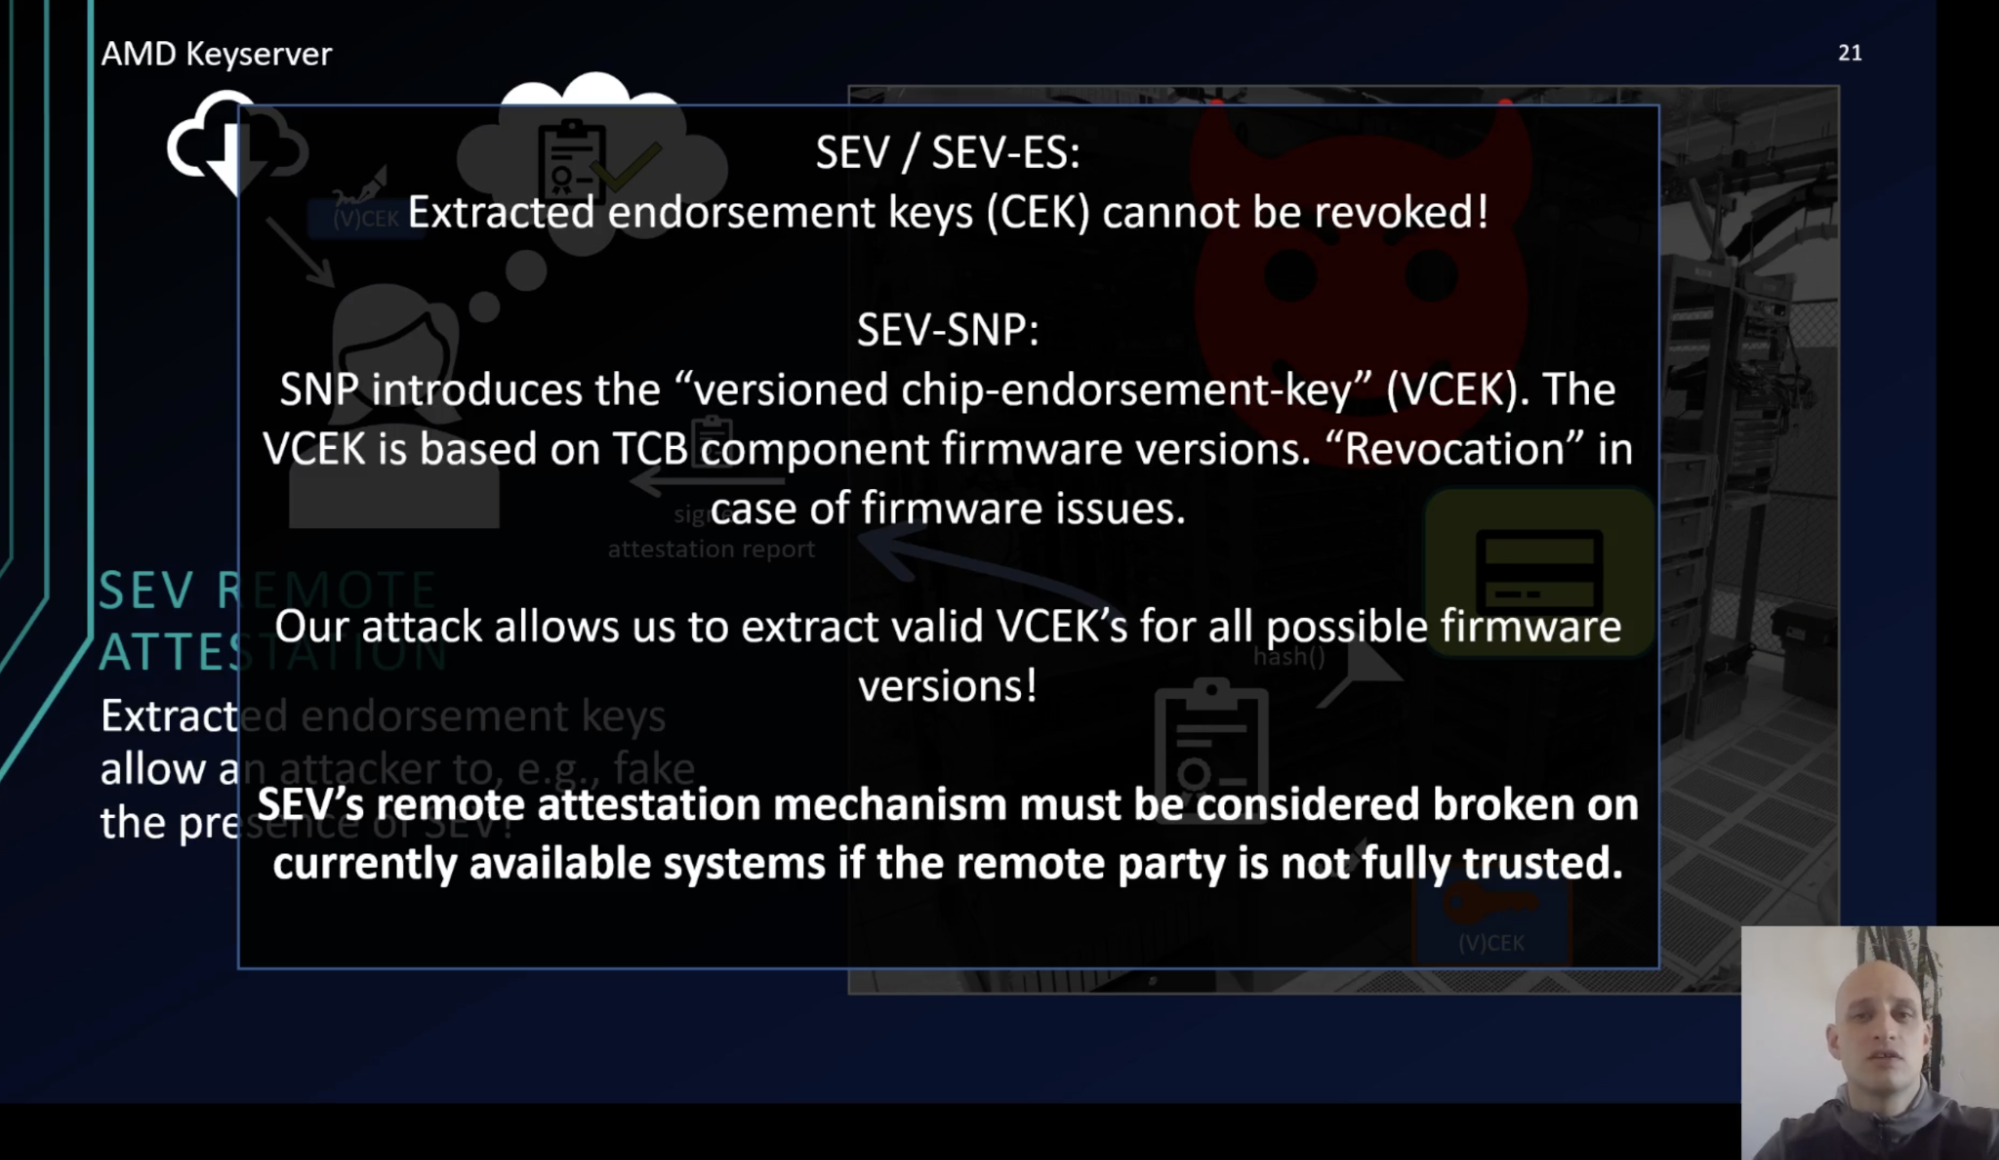
\includegraphics[width=0.6\linewidth]{buhren-1}
    \caption{Image from \cite{buhren_one_2021}}
    \label{fig:buhren-1}
\end{figure}

\begin{figure}[!ht]
    \centering
    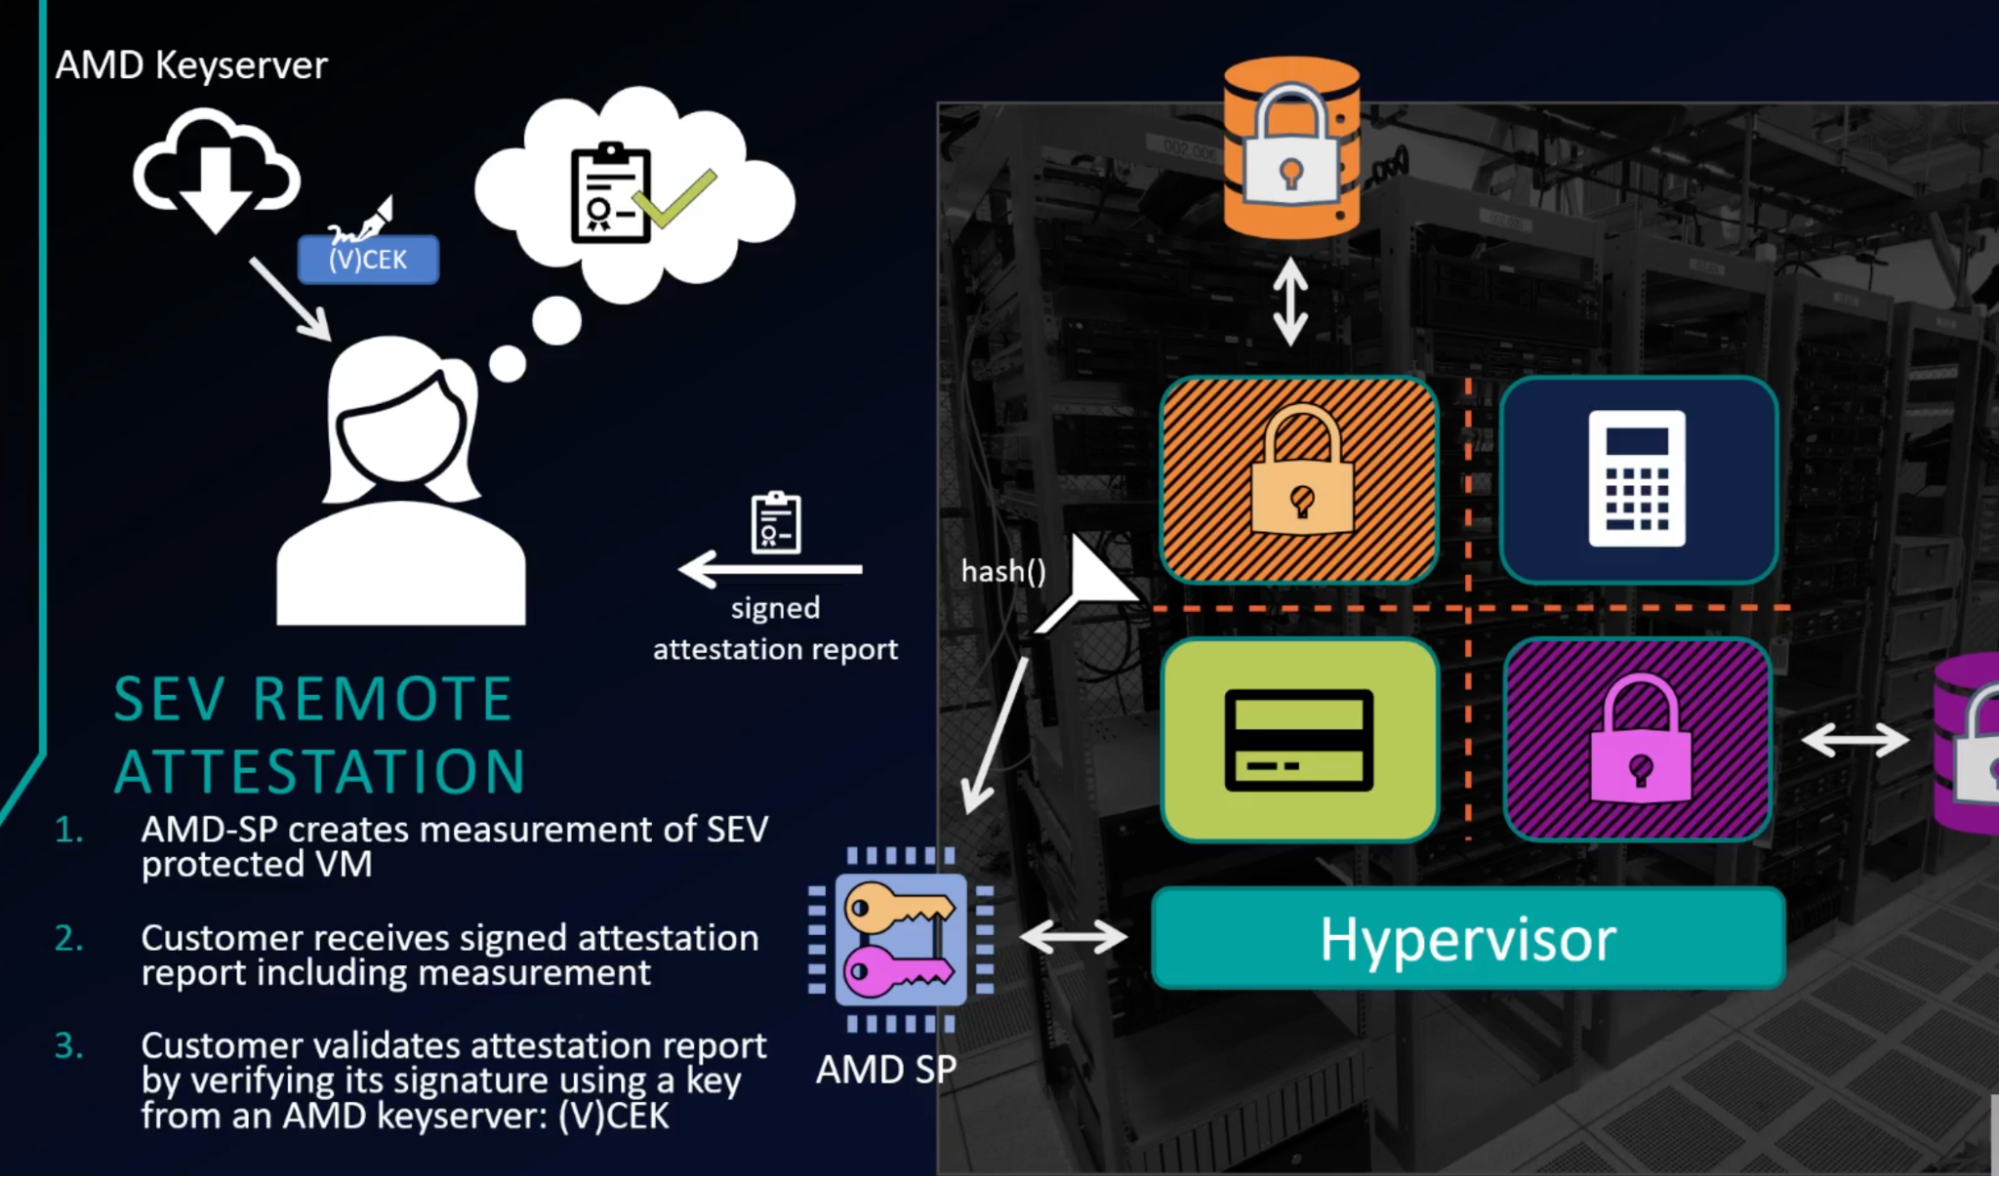
\includegraphics[width=0.6\linewidth]{buhren-2}
    \caption{Image from \cite{buhren_one_2021}}
    \label{fig:buhren-2}
\end{figure}
\begin{figure}[!ht]
    \centering
    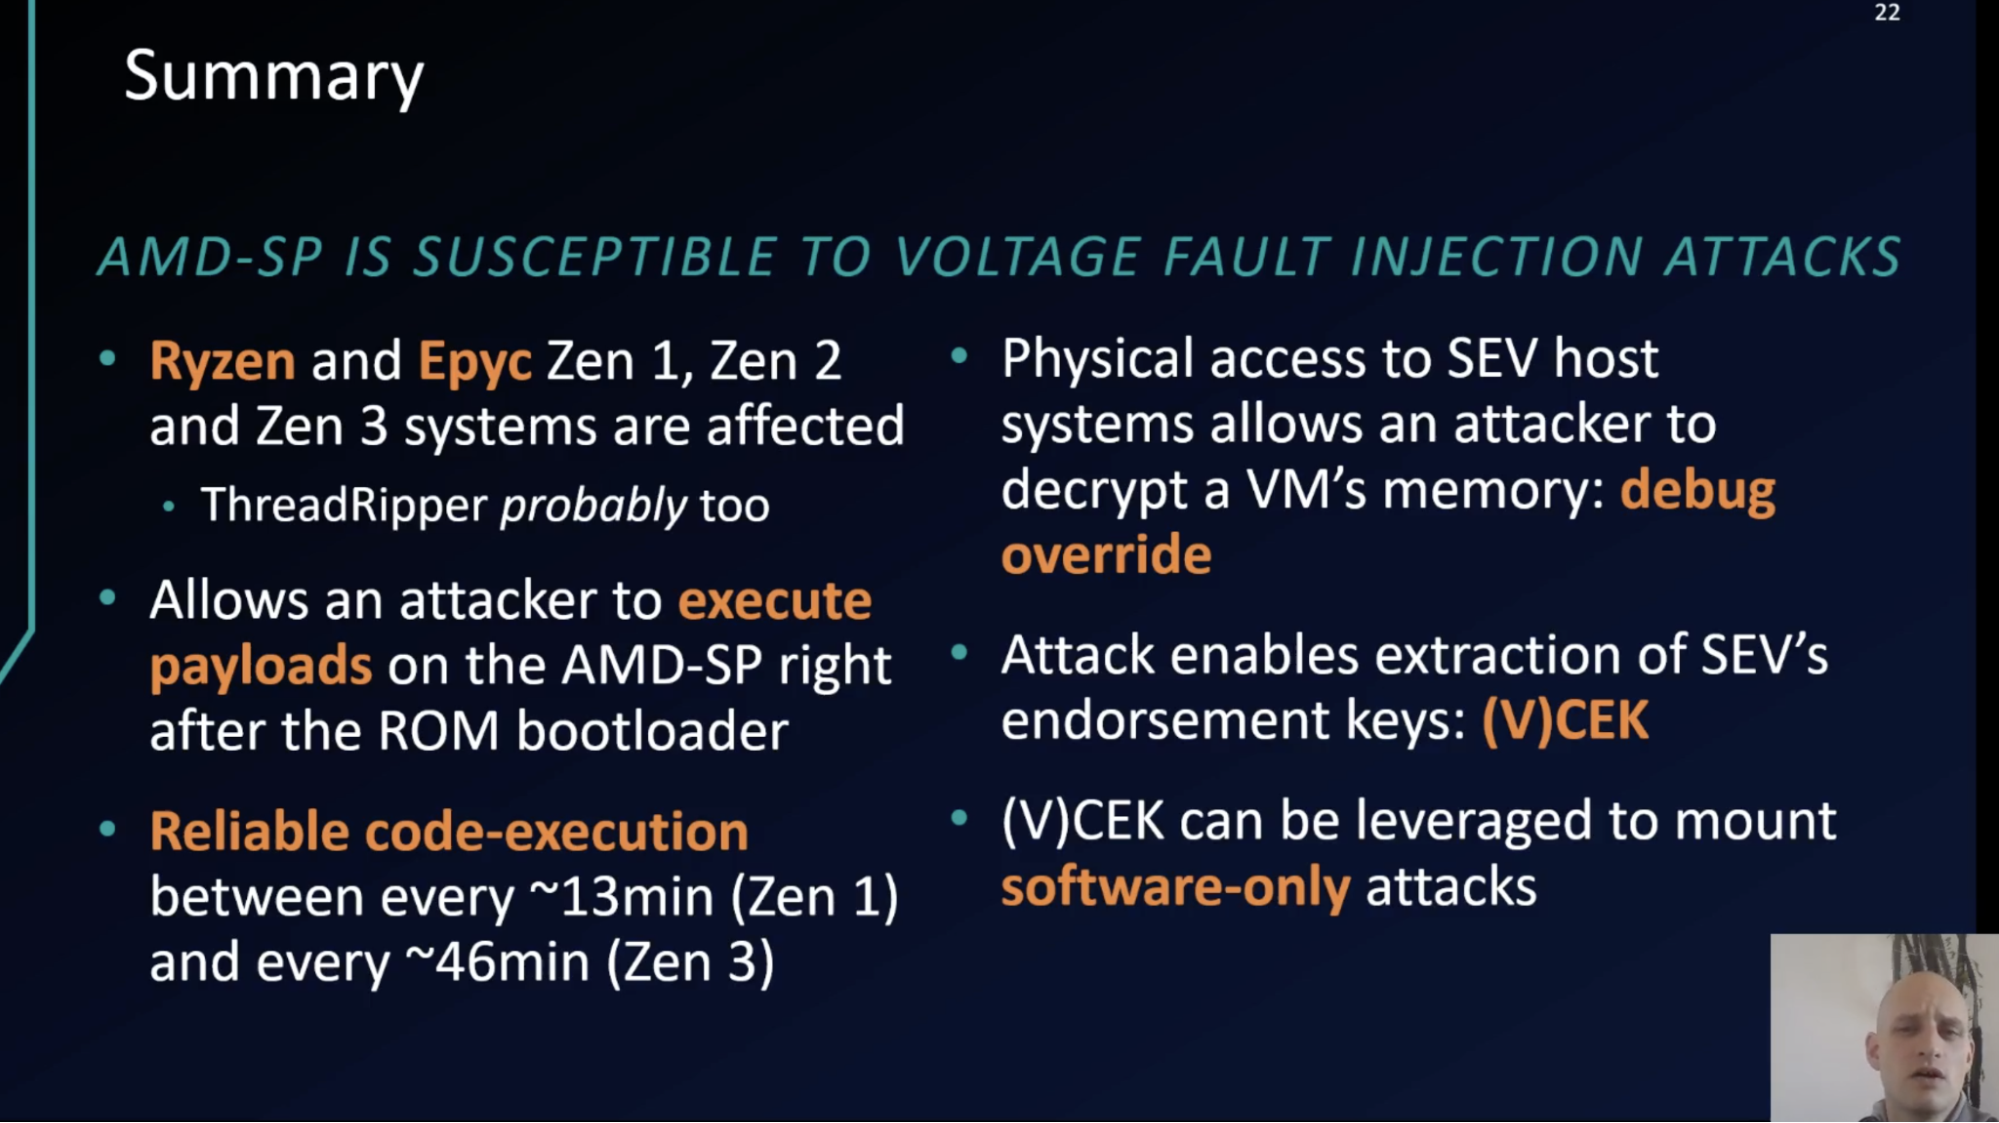
\includegraphics[width=0.6\linewidth]{buhren-3}
    \caption{Image from \cite{buhren_one_2021}}
    \label{fig:buhren-3}
\end{figure}

\newpage%!TEX root = ../main.tex

\subsection{\cite{hetzelt_via_2021} - VIA: Analyzing Device Interfaces of Protected Virtual Machines}

\textbf{VIA: Analyzing Device Interfaces of Protected Virtual Machines}

\subsubsection*{Abstract \cite{hetzelt_via_2021} }
“Both AMD and Intel have presented technologies for confidential computing in cloud environments. The proposed solutions — AMD SEV (-ES, -SNP) and Intel TDX — protect Virtual Machines (VMs) against attacks from higher privileged layers through memory encryption and integrity protection. This model of computation draws a new trust boundary between virtual devices and the VM, which in so far lacks thorough examination. In this paper, we therefore present an analysis of the virtual device interface and discuss several attack vectors against a protected VM. Further, we develop and evaluate VIA, an automated analysis tool to detect cases of improper sanitization of input recieved via the virtual device interface. VIA improves upon existing approaches for the automated analysis of device interfaces in the following aspects: (i) support for virtualization relevant buses, (ii) efficient Direct Memory Access (DMA) support and (iii) performance. VIA builds upon the Linux Kernel Library and clang’s libfuzzer to fuzz the communication between the driver and the device via MMIO, PIO, and DMA. An evaluation of VIA shows that it performs 570 executions per second on average and improves performance compared to existing approaches by an average factor of 2706. Using VIA, we analyzed 22 drivers in Linux 5.10.0-rc6, thereby uncovering 50 bugs and initiating multiple patches to the virtual device driver interface of Linux. To prove our findings’ criticality under the threat model of AMD SEV and Intel TDX, we showcase three exemplary attacks based on the bugs found. The attacks enable a malicious hypervisor to corrupt the memory and gain code execution in protected VMs with SEV-ES and are theoretically applicable to SEV-SNP and TDX.” 

\subsubsection*{Conclusion  \cite{hetzelt_via_2021} }
“We presented VIA: a framework for dynamic analysis of drivers under the threat model of a malicious HV. VIA was applied to 22 drivers in Linux 5.10.0-rc6, which covered network drivers, VirtIObased drivers, and platform drivers. The evaluation found 50 bugs from a variety of classes and initiated multiple patches to the Linux kernel. We implement Proof-of-Concept exploits for three bug classes that gain code execution or corrupt memory inside an AMD SEV-ES VM. The described exploits demonstrate how the capabilities of a malicious HV, such as control over virtual devices, fine grained control over VM execution as well as information about the VM execution state, can be used to craft reliable exploits. The majority of bugs were reported to the driver maintainers, and the security implications were responsibly disclosed.

Unlike other solutions for driver analysis, VIA carefully considers the capabilities of the HV and the semantics of the DMA API to detect more cases of improper input sanitization and anti-patterns in device programming. VIA provides a coverage-driven in-process userspace fuzzer built upon libfuzzer and LKL. Compared to existing approaches, VIA reduces setup overhead by moving the analysis into a userspace program. In combination with targeted optimizations of the userspace kernel environment, VIA drastically improves dynamic analysis throughput. To the best of our knowledge, VIA presents the first approach to analyze the device driver interface under the new threat model of protected virtual machines.

Our results suggest that many Linux device drivers do not correctly sanitize device-provided data. Under the threat model of AMD SEV-SNP and Intel TDX, this presents a serious security risk for the protected VM, which may be exploited through a software driver bug. Thus, the software operating under such a threat model should reduce the interfaces with untrusted entities and should rely on established methods for testing the remaining interfaces.” 

\newpage%!TEX root = ../main.tex

\subsection{\cite{li_crossline_2021} - CrossLine: Breaking "Security-by-Crash" based Memory Isolation in AMD SEV}

\textbf{CrossLine: Breaking "Security-by-Crash" based Memory Isolation in AMD SEV} 

\subsubsection*{Abstract \cite{li_crossline_2021}}
“AMD’s Secure Encrypted Virtualization (SEV) is an emerging security feature of modern AMD processors that allows virtual machines to run with encrypted memory and perform confidential computing even with an untrusted hypervisor. This paper first demystifies SEV’s improper use of address space identifier (ASID) for controlling accesses of a VM to encrypted memory pages, cache lines, and TLB entries. We then present the CrossLine attacks1 , a n{}ovel class of attacks against SEV that allow the adversary to launch an attacker VM and change its ASID to that of the victim VM to impersonate the victim. We present two variants of CrossLine attacks: CrossLine V1 decrypts victim’s page tables or any memory blocks conforming to the format of a page table entry; CrossLine V2 constructs encryption and decryption oracles by executing instructions of the victim VM. We discuss the applicability of CrossLine attacks on AMD’s SEV, SEV-ES, and SEV-SNP processors.”

\subsubsection*{Conclusion \cite{li_crossline_2021}}
“In conclusion, this paper demystifies AMD SEV’s ASID-based isolation for encrypted memory pages, cache lines, and TLB entries. For the first time, it challenges the “security-by-crash” design philosophy taken by AMD. It also proposes the CrossLine attacks, a novel class of attacks against SEV that allow the adversary to launch an attacker VM and change its ASID to that of the victim VM to impersonate the victim. Two variants of CrossLine attacks have been presented and successfully demonstrated on SEV machines. They are the first SEV attacks that do not rely on SEV’s memory integrity flaws.” 



\newpage%!TEX root = ../main.tex

\subsection{\cite{li_cipherleaks_2021} - CipherLeaks: Breaking Constant-time Cryptography on AMD SEV via the Ciphertext Side Channel}

\textbf{CipherLeaks: Breaking Constant-time Cryptography on AMD SEV via the Ciphertext Side Channel}

\subsubsection*{Abstract \cite{li_cipherleaks_2021}}
“AMD’s Secure Encrypted Virtualization (SEV) is a hardware extension available in AMD’s EPYC server processors to support confidential cloud computing. While various prior studies have demonstrated attacks against SEV by exploiting its lack of encryption in the VM control block or the lack of integrity protection of the encrypted memory and nested page tables, these issues have been addressed in the subsequent releases of SEV-Encrypted State (SEV-ES) and SEV-Secure Nested Paging (SEV-SNP).

In this paper, we study a previously unexplored vulnerability of SEV, including both SEV-ES and SEV-SNP. The vulnerability is dubbed ciphertext side channels, which allows the privileged adversary to infer the guest VM’s execution states or recover certain plaintext. To demonstrate the severity of the vulnerability, we present the CIPHERLEAKS attack, which exploits the ciphertext side channel to steal private keys from the constant-time implementation of the RSA and the ECDSA in the latest OpenSSL library“

\subsubsection*{Conclusion \cite{li_cipherleaks_2021}}
“This paper describes the ciphertext side channel on SEV (including SEV-ES and SEV-SNP) processors. The root causes of the side channel are two-fold: First, SEV uses XEX mode of encryption with a tweak function of the physical addresses, so that the one-to-one mapping between the ciphertext and plaintext of the same address is preserved. Second, the VM memory is readable by the hypervisor, allowing it to monitor the changes of the ciphertext blocks. The paper demonstrates the CIPHERLEAKS attack that exploits the ciphertext sidechannel vulnerability to completely break the constant-time cryptography of OpenSSL when executed in SEV-ES VMs.”

\newpage%!TEX root = ../main.tex

\subsection{\cite{li_tlb_2021} - TLB Poisoning Attacks on AMD Secure Encrypted Virtualization}

\textbf{TLB Poisoning Attacks on AMD Secure Encrypted Virtualization }

\subsubsection*{Abstract \cite{li_tlb_2021}}
“AMD’s Secure Encrypted Virtualization (SEV) is an emerging technology of AMD server processors, which provides transparent memory encryption and key management for virtual machines (VM) without trusting the underlying hypervisor. Like Intel Software Guard Extension (SGX), SEV forms a foundation for confidential computing on untrusted machines; unlike SGX, SEV supports full VM encryption and thus makes porting applications straightforward. To date, many mainstream cloud service providers, including Microsoft Azure and Google Cloud, have already adopted (or are planning to adopt) SEV for confidential cloud services.

In this paper, we provide the first exploration of the security issues of TLB management on SEV processors and demonstrate a novel class of TLB Poisoning attacks against SEV VMs. We first demystify how SEV extends the TLB implementation atop AMD Virtualization (AMD-V) and show that the TLB management is no longer secure under SEV’s threat model, which allows the hypervisor to poison TLB entries between two processes of a SEV VM. We then present TLB Poisoning Attacks, a class of attacks that break the integrity and confidentiality of the SEV VM by poisoning its TLB entries. Two variants of TLB Poisoning Attacks are described in the paper; and two end-to-end attacks are performed successfully on both AMD SEV and SEV-ES.” 


\subsubsection*{Conclusion \cite{li_tlb_2021}}
“In this paper, we present the first work to demystify AMD SEV’s insecure TLB management mechanisms and demonstrate end-to-end TLB Poisoning Attacks that exploit the underlying design flaws. Our study not only presents another vulnerability in the design of SEV, but reveals the difficulty of securely isolating TLBs with untrusted privileged software.”


\newpage%!TEX root = ../main.tex

\subsection{\cite{maarouf_cloud_2021} - Cloud Computing and Virtualization Security: A Survey}

\textbf{Cloud Computing and Virtualization Security: A Survey }

\subsubsection*{Abstract \cite{maarouf_cloud_2021}}

“Cloud computing is becoming one of the leading technologies to host Internet services as it offers flexibility for their customers besides being cost-effective for providers. Virtualization is a key technology for cloud computing as it allows hardware resources to distribute among several customers. The hypervisor (HV) is the controlling software that ensures effective isolation and security of the virtual systems. Despite its usefulness, cloud computing is neither trustworthy nor secure against local or remote attacks. To mitigate these threats, AMD Secure Encrypted Virtualization (AMD-SEV) and Intel Software Guard Extension (Intel-SGX) technologies were introduced as potential solutions by a hardware-assisted Trusted Execution Environment (TEE).

Our paper surveys several types of attacks done by either a compromised HV or a malicious tenant targeting SEV-encrypted and Intel SGX virtual machines to analyze the vulnerability in its design. We classify the literature by the position of the attacker and the purpose of attacking these VMs. We also survey different kinds of defense models that can mitigate the studied attacks.”

\subsubsection*{Conclusion \cite{maarouf_cloud_2021}}
“In this paper, we present a classification framework to categorize previous literature on cloud computing and virtualization security. Although we did not cover a substantial portion
of research papers, our framework can be used for a larger
survey, which we leave for future work. Our classification
is meant to help practitioners understand the threats against
their cloud services. We believe that expanding on the current
classification framework would prove useful to serve such a
purpose. ”



\newpage%!TEX root = ../main.tex

\subsection{\cite{mestas_exploitation_2021} - Exploitation and Mitigation of CPU Vulnerabilities}

\textbf{Exploitation and Mitigation of CPU Vulnerabilities}

\url{https://ir.library.oregonstate.edu/downloads/fj2369045}

\subsubsection*{Abstract \cite{mestas_exploitation_2021}}
“AMD SEV allows for the creation of fully encrypted virtual machines. This allows cloud computing tenants’ data to be secret to the cloud computing provider. However, it has been shown that the encryption scheme used by AMD can easily be broken. The attacker can create a copy of the virtual machine, and perform some malicious operations to gain a secret value used in the encryption scheme. They can then use this value to write and read encrypted data to and from the target virtual machine. To prevent this, we propose wrapping the insecure encryption scheme with a stronger encryption scheme. We developed a proof of concept kernel module that implements secure encryption between the user and kernel space. In addition, we discuss other CPU vulnerabilities and their potential impacts. We look at copy-on-write based side channel attacks, and introduce a method for optimizing them through making use of new CPU instructions. Also, we survey other CPU side channel attacks, and present some examples of these attacks.”

\subsubsection*{Conclusion \cite{mestas_exploitation_2021}}
“In this work, we described previous work that showed a malicious hypervisor can arbitrarily read and write private data inside of an AMD SEV protected VM. We also developed a software defense against this attack, and implemented a proof of concept of the defense. Additionally, we showed how COW based side channel attacks can be optimized through the usage of transactional memory operations on both x86 and ARM CPUs. Finally, we discussed and implemented proof of concepts for various other categories of side channel attacks. Our work has surveyed various categories of CPU vulnerabilities, and presented a defense to one vulnerability as well as an optimization to another.”


